\begin{figure}[h!]
    \begin{center}
        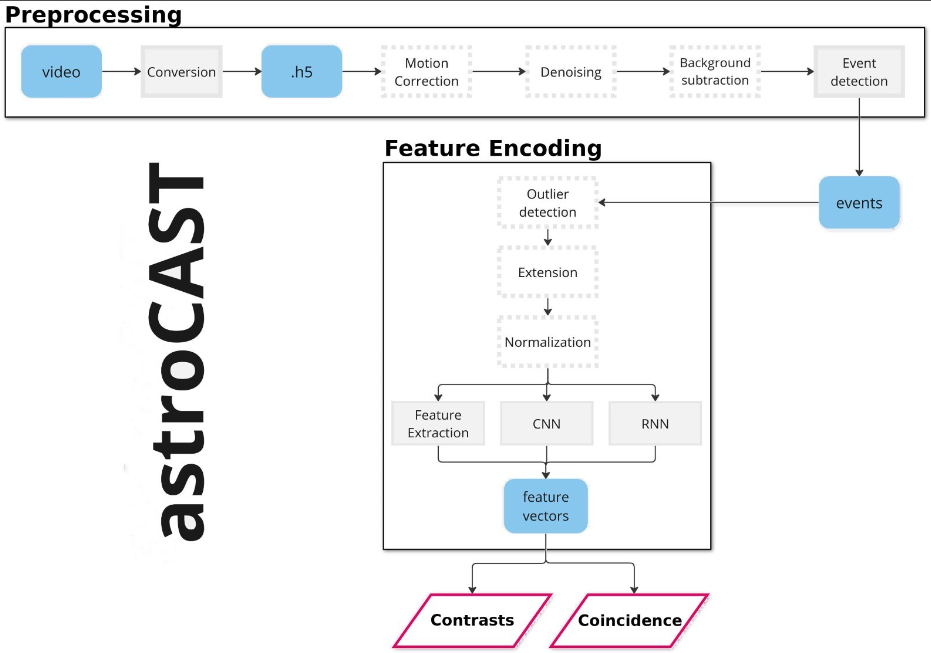
\includegraphics[width=\linewidth]{figures/1.png}
    \end{center}
    \caption{AstroCAST Pipeline Overview: First box shows how the input video is converted and processed to detect
    events. Second box shows how the detected events undergo feature extraction utilizing different approaches to
    generate feature vectors. Last steps shows how feature vectors can be analyzed to identify patterns and
    correlations. Optional steps in the pipeline are indicated by dotted boxes, and outputs at each stage are shown
    in blue. Exemplary types of experiments explained in this protocol are highlighted in red.

    }\label{fig:1}
\end{figure}

\begin{figure}[h!]
    \begin{center}
        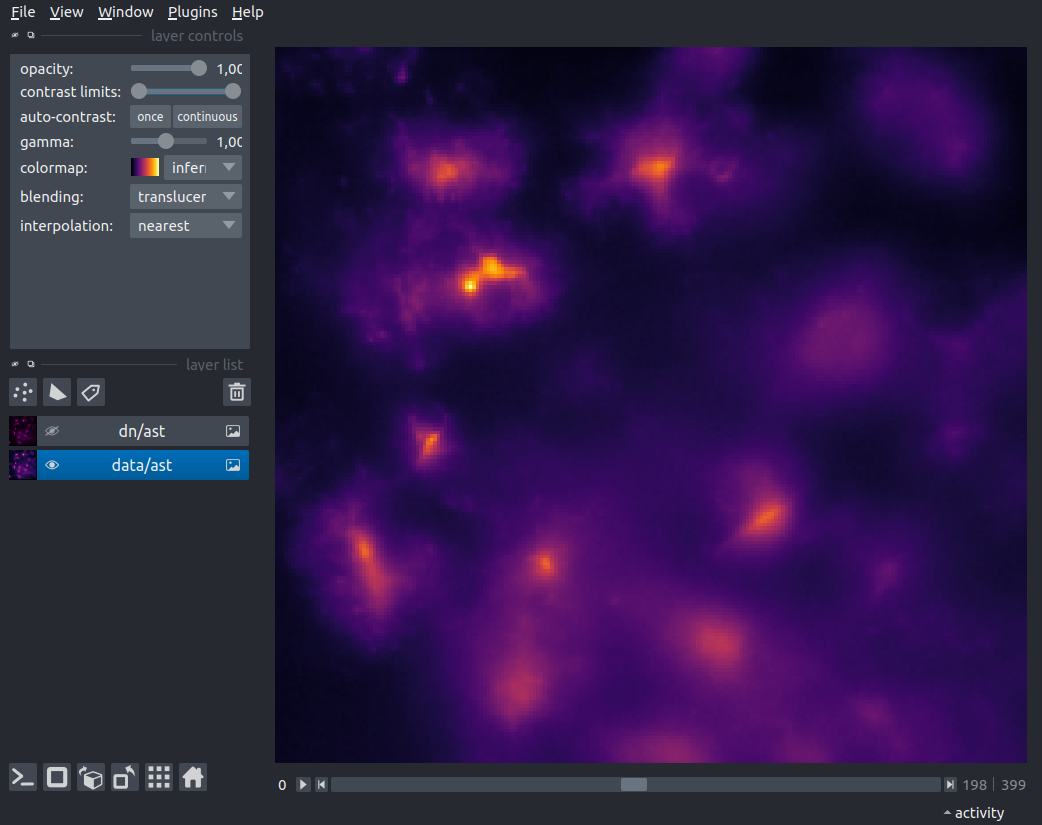
\includegraphics[width=\linewidth]{figures/2.png}
    \end{center}
    \caption{Screenshot of the \ac{GUI} displaying the converted video file of astrocytic calcium fluorescence (\ref{
        Tbl1}). The video has been downsampled and captured at a 20X magnification, focusing on the \ac{preBötC}
    region.}\label{fig:2}
\end{figure}

\begin{figure}[h!]
    \begin{center}
        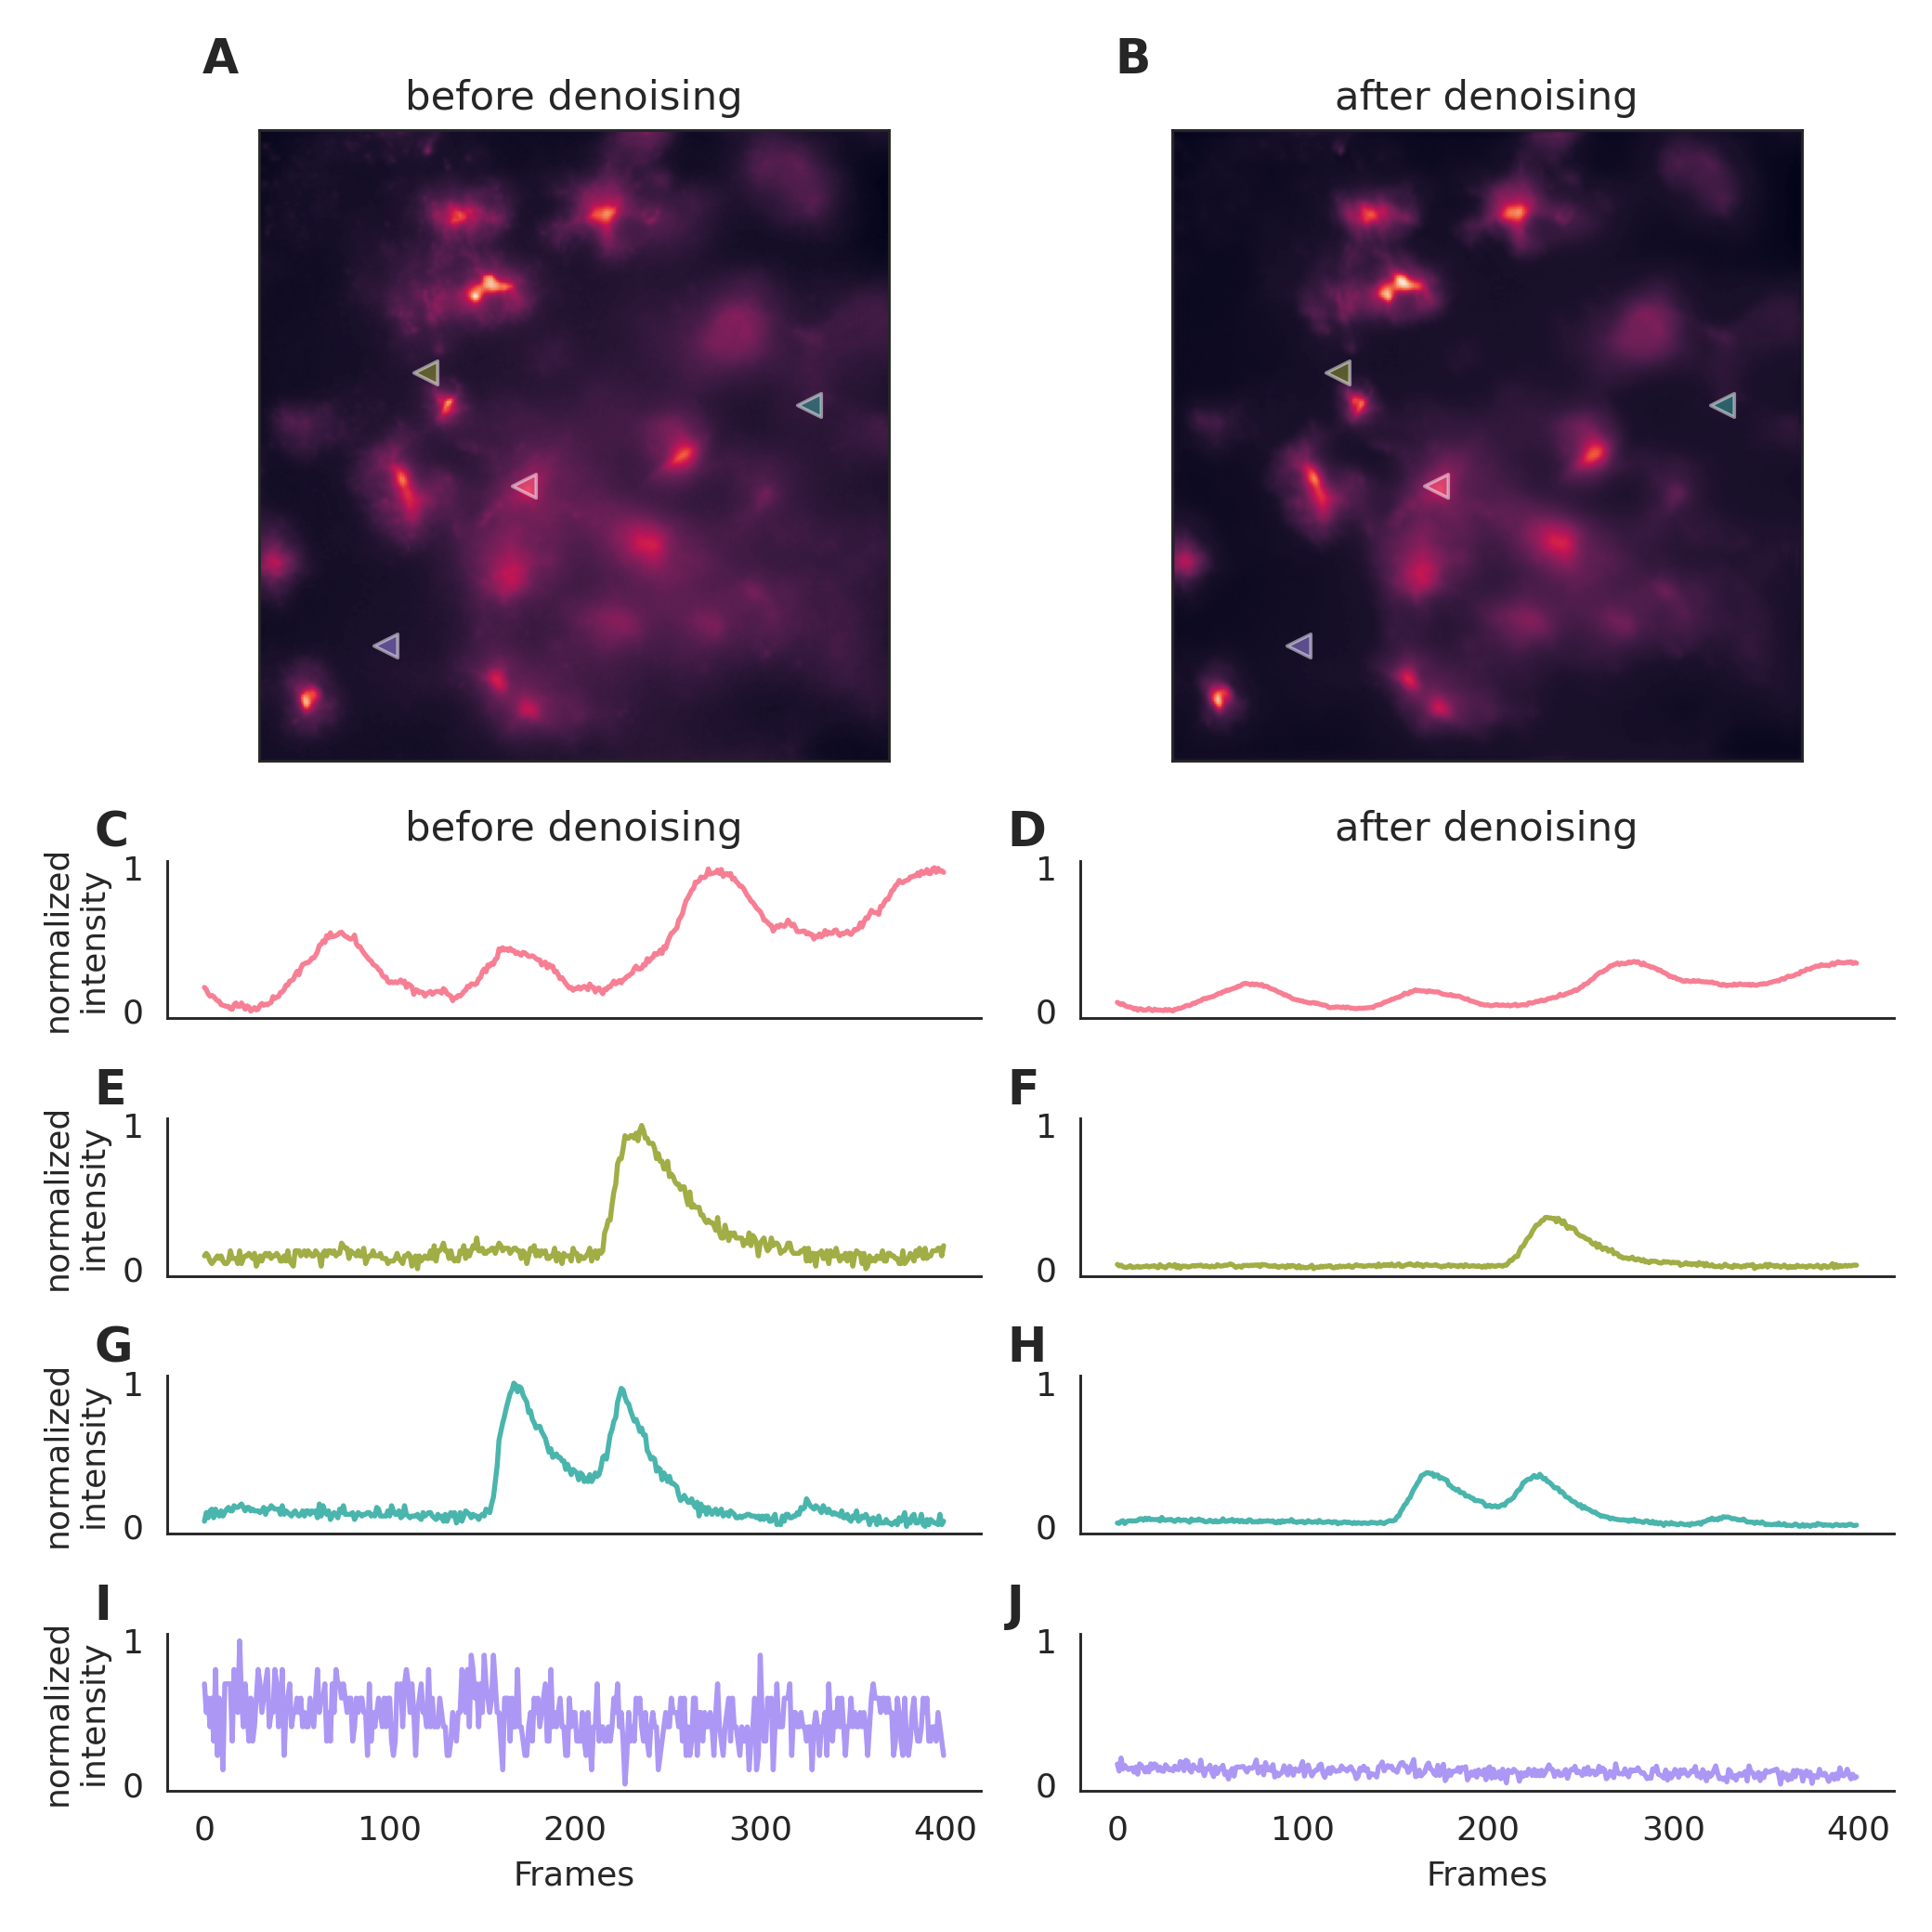
\includegraphics[width=\linewidth]{figures/3.png}
    \end{center}
    \caption{Comparative Visualization of Denoising on Video Frames and Pixel Intensity Measurements. Single frame (
        512x512 pixels) before denoising (left panel), showing notable background, and the corresponding frame after
        the application of a denoising algorithm, showing reduced background and enhanced clarity (middle panel).
        Pixel intensity traces from four selected points (right panel, P0-P3) in the video frame before denoising,
        displaying the variation over 200 frames. Right Plot) Pixel intensity traces for the same points after
        denoising, indicating a more stable intensity profile, while retaining features of the signal. The denoising
        algorithm was applied to a (128, 128) field of view with a configuration of 5 frames, each bordering the
        target frame, and no gap frames. The denoiser, trained for 50 epochs on a custom dataset, had a learning rate
        of 0.0001, momentum of 0.9, 3 layer stacks (n\_stacks), and 64 kernels of size 3 in the first layer without
        batch normalization. Inference involved a 10-pixel overlap in each direction with 'edge' padding. The test
        and validation were conducted using the same custom training dataset.
    }\label{fig:3}
\end{figure}

\begin{figure}[h!]
    \begin{center}
        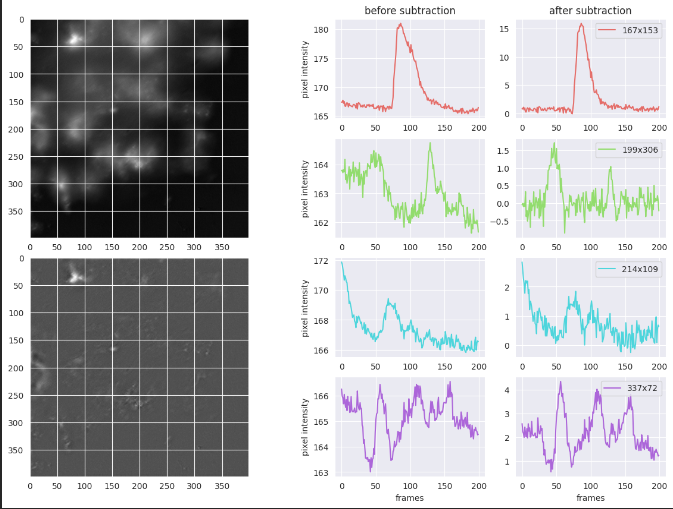
\includegraphics[width=\linewidth]{figures/4.png}
    \end{center}
    \caption{Background Subtraction in Fluorescence Imaging Analysis. Comparative analysis of fluorescence images and
    pixel intensity traces before (top left) and after background subtraction (bottom left). Pixel intensity over
    time (right panels). These plots reveal the background noise reduction, where post-subtraction y-axis values are
    near zero, indicating effective subtraction. Event shapes remain consistent, verifying reliable preservation of
    events. Notably, the second panel (green) slightly alters the signal strength of events, underscoring the
    importance of careful parameter optimization or exclusion of this step if it compromises data fidelity. Please
    refer to Video S2\ref{} for a dynamic visualization.}\label{fig:4}
\end{figure}

